\documentclass[10pt, compress]{beamer}

\usetheme{m}

\usepackage{booktabs}
\usepackage[scale=2]{ccicons}
\usepackage{minted}
\usepackage{textcomp}

\usepgfplotslibrary{dateplot}

\usemintedstyle{trac}

\title{Compact Name-Independent Routing with Minimum Stretch}
\subtitle{}
\date{\today}
\author{Jonas Brunsgaard and Henrik Bendt}
\institute{DIKU}

\begin{document}

\maketitle

\section{Lets talk a bit about routing}
\begin{frame}[fragile]
  \frametitle{Routing Scheme}
    A routing scheme is a distributed algorithm that allows any
    source node to route messages to any destination node, given
    destination node's name

    \begin{description}
        \item[Input] a network $G$ (a weighted connected graph)
        \item[Output] a routing scheme for G
    \end{description}
\end{frame}

\begin{frame}{XY-routing}
  \begin{figure}
    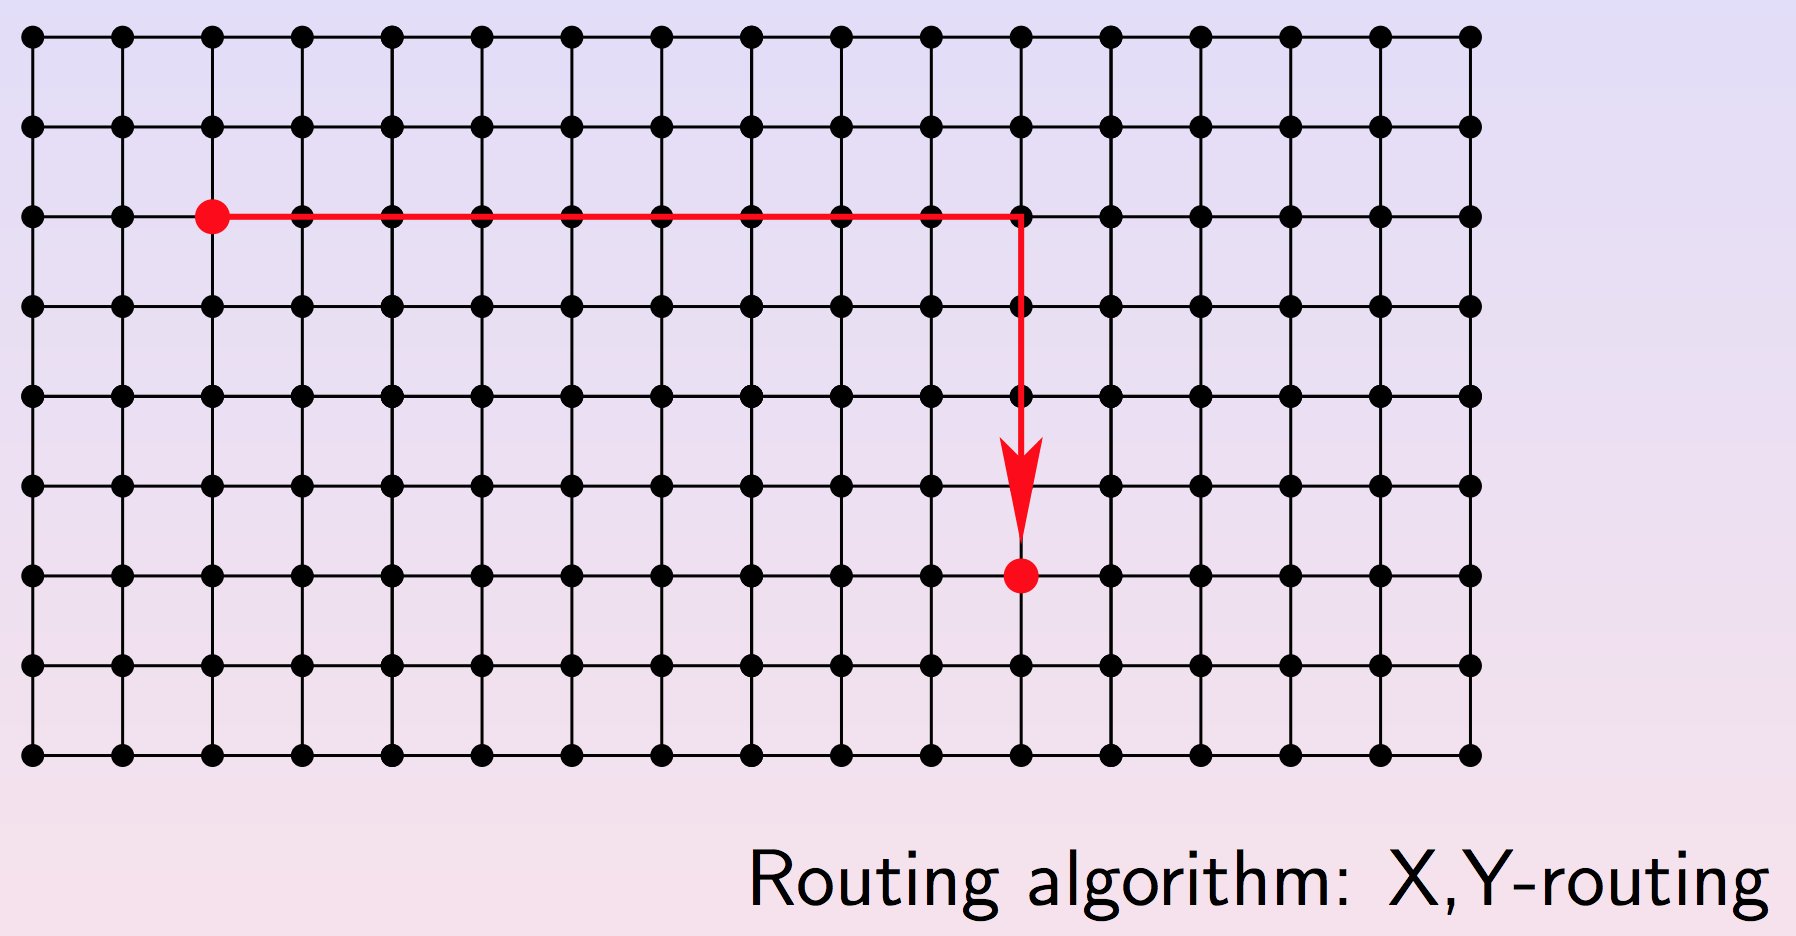
\includegraphics[scale=0.3]{images/xyrouting.png} 
  \end{figure}
\end{frame}

\begin{frame}[fragile]
  \frametitle{Routing Scheme}
     
  \begin{block}{Example: Trivial routing on min cost paths}
      \begin{itemize}
        \item On each node, for each of the possible $(n-1)$ destinations,
        store a port number leading to the next node on a min cost path to the
        destination.
        \item Requires each node to store $\Omega (n\; log\; n)$ bits.
        \item Does not scale very well.
      \end{itemize}
  \end{block}
\end{frame}

\begin{frame}[fragile]
  \frametitle{Minimizing parameters}
  When working with routing, two factors are normally of interest:
  \begin{description}
    \item[Stretch] The max ratio over all source-destination pairs between the
        cost of the path taken by the routing scheme and the cost of a min
        cost path.
    \item[Memory] The max number of bits over all nodes stored for the routing
        scheme. (ballanced is preferred)
  \end{description}
\end{frame}

\begin{frame}[fragile]
  \frametitle{Labeled Routing or Name-Independent Routing}

  In labeled routing we can choose a label for each vertex.
  Lets use coordinates. Now we can easily route. If an aversery
  label the vertices randomly, routing gets harder.

  \begin{figure}
    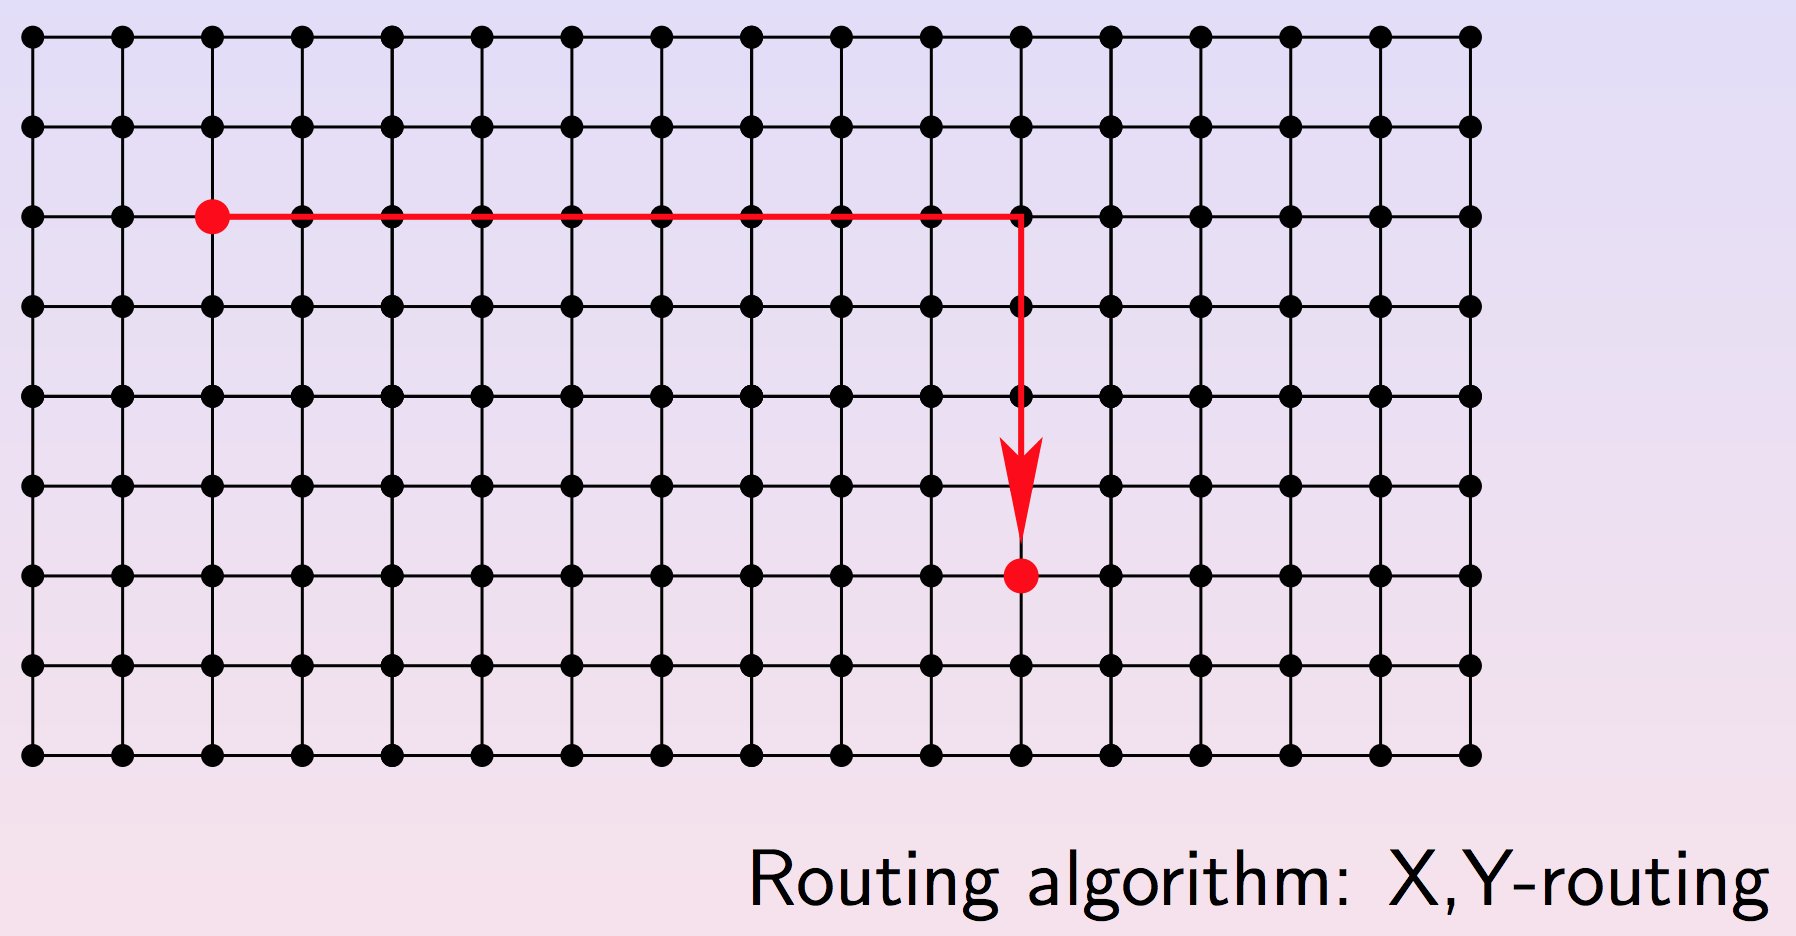
\includegraphics[scale=0.3]{images/xyrouting.png} 
  \end{figure}
\end{frame}

\section{Okay, I get routing, what is the article about?}

\begin{frame}[fragile]
  \frametitle{Name-Independent Rounting with min stretch}
    Given a weighted undirected network with arbitrary node names, we present
    a compact routing scheme, using a $\tilde{O}(\sqrt{n})$ space routing
    table at each node and routing along paths of stretch 3.

    It is known that no compact routing using $o(n)$ space per node can route
    with stretch below 3. Also, it is known that any stretch below 5 requires
    $\Omega(\sqrt{n})$ space per node.
\end{frame}

\begin{frame}[fragile]
  \frametitle{Setup}
    Consider an $n$-node weighted undirected graph $G=(V,E,\omega)$.

    Each node $v\in V$:
    \begin{itemize}
        \item is given a unique name with $O(log\; n)$ bits.
        \item each outgoing edge is given a unique port name in $\{1,\dots,deg(v)\}$.
    \end{itemize}
\end{frame}



\section{The Stretch 3 Scheme}

\begin{frame}[fragile]
  \frametitle{Vicinity Balls}

  For every integer $k \geq 1$, and for a node $u \in V$, let the \textit{vicinity} of $u$, denoted by $B_k(u)$, be the set consisting of $u$ and the $k$ closest nodes to $u$.

  Set $k=[4 \sqrt{n}log\; n]$ and denote $B(u) = B_k(u)$.\\
  Denote $b(u)$ the radius of $B(u)$, $b(u)=max_{w\in B(u)} d(u,w)$.

  %HB

\end{frame}

\begin{frame}[fragile]
  \frametitle{Coloring}

  Partition nodes into the color sets $C_1,\dots,C_{\sqrt{n}}$, with the following properties:
  \begin{enumerate}
    \item Every color-set has at most $2 \sqrt{n}$ nodes.
    \item Every node has in its vicinity at least one node from every color-set.
  \end{enumerate}

  If node $u\in C_i$, it has ``color $i$''. Denote $c(u)=i$.

  This can be constructed in polynomial-time.

  If every node independently chooses a random color, the properties holds with high probability.

  %HB

\end{frame}

\begin{frame}[fragile]
  \frametitle{Hashing Names To Colors}

  Assuming a mapping $h$ from node names to colors is balanced such that at most $O(\sqrt{n})$ names map to the same color.

  Each node $u\in V$ should be able to compute $h(w)$ for any destination $w$.

  %HB

\end{frame}

\section{Stretch 3 for Complete Graph}

\begin{frame}[fragile]
  \frametitle{Storing}

  Every node $u$ stores the following:

  \begin{enumerate}
    \item The names of all the nodes in the vicinity $B(u)$ and what port number to use to reach them.
    \item The names of all nodes $v$ such that $c(u)=h(v)$ and what port number to use to reach them.
  \end{enumerate}

  %HB

\end{frame}


\begin{frame}[fragile]
  \frametitle{Routing}

  Routing from $u$ to $v$:
  \begin{enumerate}
    \item If $v\in B(u)$ or $c(u)=h(v)$, then $u$ routes directly to $v$ with stretch 1 (i.e. min cost)
    \item Otherwise, $u$ forwards the packet to $w\in B(u)$ such that $c(w)=h(v)$. Then from $w$ the packet goes directly to $v$.\\
        The stretch is at most $3$ since $d(u,w) + d(w,v) \leq d(u,v)+2d(u,v)$.
  \end{enumerate}

  %HB

\end{frame}


\section{Stretch 3 Scheme (for all graphs)}

\begin{frame}[fragile]
  \frametitle{Routing on Trees}
    \begin{block}{Fraigniaud and Gavoille 2001, Thorup og Zwick 2001B}
        \begin{quote}
        For every weighted tree T with n nodes there exists a labeled routing
        scheme that, given any destination label, routes optimally on T from any
        source to the destination. The storage per node in T, the label size, and
        the header size are $O(log2 n/ log log n)$ bits. Given the information of
        a node and the label of the destination, routing decisions take constant
        time.
        \end{quote}
    \end{block}
    Okay, seems good. So we can route with these properties. Hurra!
\end{frame}

\begin{frame}[fragile]
  \frametitle{Landmarks}
  \begin{itemize}
    \item Designate one color to be the landmark color.
    \item Let $L$ denote the set of nodes with this color.
    \item Because of the way coloring works:
    \begin{itemize}
        \item $|L| \leq 2 \sqrt{n}$
        \item For every $v\in V$, $B(v)\cap L \neq \emptyset$
    \end{itemize}
    \item For a node $v\in V$, let $\ell_v$ denote the closest landmark node in $B(v)$.
  \end{itemize}
\end{frame}

\begin{frame}[fragile]
  \frametitle{Partial shortest path trees}
  For any node $u$, let $T(u)$ denote a singlesource minimum-cost-path tree
  rooted at $u$. In a partial shortest path tree, every node $v$ maintains
  $\mu(T(u),v)$ if and only if $u \in B(v)$. Notice that the set of nodes that
  maintain $\mu(T(u),\dot)$ is a subtree of $T(u)$ that contains $u$
  \begin{block}{Lemma 3.4}
    \begin{quote}
    If $x \in B(y)$, then given the label $\lambda(T(x), y)$, node $x$ can
    route to node $y$ along a minimum cost path
    \end{quote}
  \end{block}
\end{frame}

\begin{frame}[fragile]
  \frametitle{Storing}

  Every node stores:
  \begin{enumerate}
    \item For every $w\in B(u)$, the name $w$ and the port name $u\rightarrow y$, where $(u\rightarrow y)$ is the port number to use to get to node $y$, which is the next hop on a min cost path from $u$ to $w$.
    \item For every landmark node $\ell \in L$, routing information $\mu(T(\ell),u)$ and label $\lambda(T(\ell),\ell)$ of the tree $T(\ell)$.
    \item For every node $x\in B(u)$, routing information $\mu(T(x),u)$ of the tree $T(x)$.
\end{enumerate}

  %JB
  %TODO 3.8, (1)..(3)

\end{frame}

\begin{frame}[fragile]
  \frametitle{Storing}
    4. For every node v such that $c(u) = h(v)$, store one of the following two options that produces the minimum cost path out of the two:

    \begin{enumerate}
    \item[a] Store the labels $<\lambda(T (\ell_v), \ell_v ), \lambda(T (\ell_v), v)>$. The routing path in this case would be from $u$ to $\ell_v \in B(v)$ using $\lambda(T (\ell_v), \ell_v)$ on the tree $T (\ell_v)$, and from $\ell_v$ to $v$ using $\lambda(T (\ell_v), v)$ on the same tree $T (\ell_v)$.
    \end{enumerate}

  %JB
  %3.8, (4)(a),(b)

\end{frame}

\begin{frame}[fragile]
  \frametitle{Storing}
    \begin{enumerate}
    \item[b] Let $P(u, w, v)$ be a path from u to v composed of a minimum cost path from $u$ to $w$, and of a minimum cost path from $w$ to $v$ with the followingproperties: $u \in B(w)$, and there exists an edge $(x, y)$ along the minimum cost path from $w$ to $v$ such that $x \in B(w)$ and $y \in B(v)$. If such paths exists, choose the lowest cost path $P(u, w, v)$ among all these paths and store the labels $<\lambda(T (u), w), x, (x → y), \lambda(T (y), v)>$.\\
    The routing path in this case would be from $u$ to $w$ on $T(u)$ using $\lambda(T (u), w)$. This part is possible by Lemma 3.4 on $u \in B(w)$. Then from $w$ to $y$ since $x \in B(w)$ and the port number $(x \rightarrow y)$ is stored. Finally from $y$ to $v$ on $T(y)$ using $\lambda(T (y), v)$. This part is possible by Lemma 3.4   on $y \in B(v)$.
    \end{enumerate}

  %JB
  %3.8, (4)(a),(b)
\end{frame}


\begin{frame}[fragile]
  \frametitle{Routing}
  \begin{block}{Routing from u to v is done in the following manner:}
    \begin{enumerate}
        \item If $v \in B(u)$ or $v \in L$ ($v$ is a landmark node) or $c(u) =
            h(v)$, then $u$ routes to $v$ using its own information.
        \item Otherwise, $u$ forwards the packet to $w \in B(u)$ such that
            $c(w) = h(v)$. Then from $w$ the packet goes to $v$ using $w$’s
            routing information.
    \end{enumerate}
  \end{block}


\end{frame}


\begin{frame}[fragile]
  \frametitle{Routing}
  \begin{block}{Routing from u to v is done in the following manner:}
    \begin{enumerate}
        \item If $v \in B(u)$ or $v \in L$ ($v$ is a landmark node) or $c(u) =
            h(v)$, then $u$ routes to $v$ using its own information.
        \item Otherwise, $u$ forwards the packet to $w \in B(u)$ such that
            $c(w) = h(v)$. Then from $w$ the packet goes to $v$ using $w$’s
            routing information.
    \end{enumerate}
  \end{block}

\end{frame}


\begin{frame}[fragile]
  \frametitle{Theorem 3.5}
    Let $s,t\in V$ be any two nodes. The route of the scheme from $s$ to $t$ has stretch at most 3.

    Proof: Three cases to consider.
\end{frame}

\begin{frame}[fragile]
  \frametitle{Analysis}
    The taget is inside the source vicinity.
    \begin{enumerate}
        \item[1] If $t\in B(s)$ or $t\in L$, then $s$ routes on a minimum cost path directly to $t$.
    \end{enumerate}
\end{frame}

\begin{frame}[fragile]
  \frametitle{Analysis}
    The source and target vicinities are far apart.
    \begin{enumerate}
        \item[2] let $z$ be a node such that $z\in B(s)$ and $c(z)=h(t)$. For the case $c(s)=h(t)$, set $z=s$. Let $p(z,t)$ be the cost of the path chosen by $z$ as the lowest cost path from $z$ to $t$ (from options 4(a) and 4(b)).

        On every min cost path from $s$ to $t$ there is a node $y$ such that $y\not\in B(s)$ and $y\not\in B(t)$. In this case, $b(s)+b(t)\leq d(s,t)$.

        From 4(a) the cost $d(s,z)+p(z, t)$ of the path taken by the routing scheme is bounded by the cost of the path $s\leadsto z\leadsto \ell_t\leadsto t$, where $u\leadsto v$ is the min cost path from $u$ to $v$.\\
        Thus $d(s,z)+p(z,t) \leq d(s,z)+d(z,\ell_t)+d(\ell_t,t) \leq b(s) + [d(s,t) + b(t)] + b(t) \leq 3d(s,t)$.
    \end{enumerate}
\end{frame}

\begin{frame}[fragile]
  \frametitle{Analysis}
    The source and atarget vicinities are close.
    \begin{enumerate}
        \item[3] There exists a min cost path in which every node is in $B(s)\cup B(t)$. Let $(x,y)$ be an edge on this path such that $x\in B(s)$ and $y\in B(t)$. From 4(b), the cost $d(s,z)+p(z,t)$ of the path taken is bounded by the cost of path $s\leadsto z\leadsto x\rightarrow y \leadsto t$.\\
        Thus $d(s,z)+p(z,t) \leq d(s,z) + d(z,s) + d(s,t) \leq b(s)+b(s)+d(s,t)\leq 3d(s,t)$.
    \end{enumerate}
\end{frame}

\section{Results}

\begin{frame}[fragile]
  \frametitle{Results}

  \begin{description}
    \item[Stretch] 3
    \item[header size] $O(log^2/log\;log\;n)$ bits
    \item[Routing information per node] $\tilde{O}(\sqrt{n})$ bits
    \item[Routing] $O(1)$ time
    \item[Construction time] $\tilde{O}(n|E|)$
  \end{description}

  %HB
  %TODO present section 1.1, i.e. construction time, runing time, space complexity
\end{frame}

\begin{frame}[fragile]
  \frametitle{Results}
  Improves the stretch of Arias et al. [2003] from 5 to 3, the known lower bound.

  Answers the open problem from 1989 [Awerbuch et al. 1990].

  %HB
\end{frame}

%Results
%Compare to other routing solutions (as done in the introduction?)

%Other?
%Examples?


\end{document}
